\documentclass[times, utf8, zavrsni]{fer}
\usepackage{booktabs}
\usepackage[numbers]{natbib}
\usepackage{algorithmic}
\usepackage{algorithm}
\usepackage{amsmath}
\usepackage{graphicx}
\usepackage{subfigure}
%\usepackage{hyperref}

\begin{document}

\thesisnumber{2037}

\title{Speed Limit Enforcement using Artificial Neural Networks}

\author{Leo Osvald}

\maketitle%

% Dodavanje zahvale ili prazne stranice. Ako ne želite dodati zahvalu, naredbu ostavite radi prazne stranice.
\zahvala{}

\begin{sazetak}
Cilj ovog rada jest istražiti jedan mogući sustav za detekciju prekoračenja
brzine vozila koji koristi slike vozila snimljene na dvije kontrolne točke kako bi
detektirao prekoračenje brzine. Naglasak rada je bio na ekstrakciji značajka iz
slika, kao i na pripremanju istih za ulaz u umjetnu neuronsku mrežu. Također,
ravijen je i analiziran algoritam sparivanja baziran na vjerojatnostima
podudaranja slika. Nadalje, napravljena je softverska implementacija dijela
sustava. U praktičnom dijelu, značajke s najboljim svojstvima razlučivosti, prehodno ustanovljene
statističkom analizom, dovedene su na ulaze neuronskih mreža. Konačno, proveden
je niz testova s ciljem validacije korištene metode.

\kljucnerijeci{podudaranje slika, detekcija brzine, obrada slike, ekstrakcija
značajki, algoritam sparivanja, umjetne neuronske mreže}
\end{sazetak}
\engtitle{Speed Limit Enforcement using Artificial Neural Networks}
\begin{abstract}

The purpose of this thesis was to investigate a system for vehicle speed limit
detection which uses vehicle image images captured at the checkpoints in order
to detect speed limit violation. The focus was on feature extraction from the
captured images as well as their preparation for being used as inputs of one or
more artificial neural networks. In addition, the matching algorithm which
matches the images based on their match probability, previously computed by the
use of artificial neural networks, is developed and thoroughly analyzed.
Moreover, software implementation of a part of the system was made. In the
experimental part, the best discriminating features determined by statistical
analysis were used as inputs in artificial neural networks. Finally, a
series of tests was carried out to validate the method.

\keywords{image matching, speed limit detection, image processing, feature
extraction, matching algorithm, artificial neural networks}
\end{abstract}

\tableofcontents

\chapter{Introduction}
In the present day, traffic safety is of great importance, given the large
numbers of vehicles. For this reason, various systems are in place to monitor or
enforce traffic safety. As traffic grows in pace, size and complexity, automatic
or semi-automatic systems tend to be more useful as those can offer immediate
feedback, high availability and scalability. In this thesis, one such system
will be considered.

More specifically, this system will deal with speed limit violations in traffic,
because speed limit enforcement is one of factors contributing to higher road
safety. Existing systems generally use a common approach: vehicle speed is
measured at points along a road, often utilizing speed radars or cameras. The
proposed system shares some of the characteristics of common ones, but
provides some unique properties. 

The requirements of the proposed system are:
\begin{enumerate}
  \item identify the violators with minimum fail rate
  \item store the proof of speed limit violation for each violator
  \item provide a means of semi-automatic reporting of violators
  \item detect violators who are familiar with the positions of radars
  \item the system accuracy is not affected by traffic conditions, including
  	sudden congestions, extremely low or high traffic etc.
\end{enumerate}
The first two requirements are self-explanatory and every serious
speed detection system meets them. Note that fail rate depends on two
variables: the number of misdetected speed limit violations (i.e. false positive) and the number of vehicle
which exceeded the speed limit but were not detected (i.e. false negative).
The latter is more problematic, since the former still leaves a the possibility
of canceling the consequences of misdetection. For instance, the system can just
wait for a user action to confirm the suspect vehicle.

As regards the third requirement, the system must prepare the information
about violators so that they could be reported with minimal effort from the
user. The reporting of violators can be either automatic or semi-automatic.
Automatic reporting implies that the system is able to automatically
identify the vehicle, since this is a necessary step to take legal action
against the driver of the vehicle. Semi-automatic reporting requires an
additional ``review \& confirm'' step, where the user is presented the image of
the violator, along with the details of violation, and then decides whether the
speed limit was exceed.

The fourth requirement deserves a closer inspection. The majority of speed
detection systems use radars to detect violators. A notable disadvantage of
this method is that the driver of the vehicle, if informed on time, can just
drop the speed of the vehicle in the right moment and later, once the vehicle
passes the sensor, increase the speed above the limit without any risks of being
detected. Of course, this problem can be reduced by periodically changing the
positions of sensors on various sections of the road, but the main problem still
persists. Moreover, this repositioning is usually expensive. 

Finally, the system should be robust to various changes in traffic conditions.
The systems with sensor-based detection methods such as radar might have a
problem here, especially in the low-headway situations where vehicles pass one
after another in close time intervals.

\chapter{Speed Limit Enforcement using Artificial Neural Networks}

In this chapter, a speed limit enforcement system based on artificial neural
networks (referred to as SLESANN) will be discussed.

\section{Principle of operation}

%\subsection{System architecture}
The system comprises a central unit and at least two checkpoints. The
checkpoints are places on the road equipped with a camera, a radar speed gun and
a small computer. The components are connected in such a way that each 
checkpoint can independently communicate with the central unit. 
The communication is usually one-way, from checkpoints to the central unit.

When a vehicle passes through a checkpoint, the camera takes the picture of it
and sends it to the central processing unit. The system keeps track of this
passes and associates the image of each vehicle with the timestamp denoting the
time when the vehicle passed through the checkpoint.

Using the information above, it is possible to track the vehicles. 

If a vehicle passes two adjacent checkpoints and those checkpoints are connected
by a unique one-directional path, it can be inferred that a vehicle traversed
the section defined by those two checkpoints (referred to as the monitored
section). The basic scenario is a section of a one-way road with no
intersections, with a checkpoint on each end of the section (i.e. exit point). A
more practical scenario with four checkpoints monitoring the sections of three
different roads is shown in figure \ref{fig:checkpoints}.

\begin{figure}[htb]
\caption{Configuration of 4 checkpoints monitoring three sections of a road}
\centering
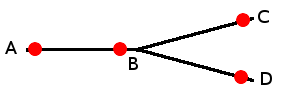
\includegraphics[width=0.4\textwidth]{images/checkpoints}
\label{fig:checkpoints}
\end{figure}

In general, the checkpoints can be placed arbitrarily on various sections of one
or more roads, but the tendency is to place them on the roads with a small
number of intersections in order to minimize the total number of checkpoints
needed to ensure there is no short route which bypasses any of the checkpoints.

Strictly speaking, the monitored sections have one or more exit points in the
middle. The system would still operate, but it would fail to detect the speed
limit violations more often. This is so because of the simple fact that
potential speed limit violators could escape by leaving the section through an
unmonitored exit point somewhere in the middle.
 
Finally, whenever a vehicle enters a section of road between two checkpoints and
leaves it, the corresponding timestamps can be used to check if the vehicle has
exceeded the speed limit. The method of detecting violators will be discussed
further in this section.

\subsection{Pass detection}
Whenever a vehicle passes a checkpoint, the checkpoint has to inform the central
unit. This is detected with a radar speed gun. Once the speed of the vehicle is
known, the exposition of the camera is adjusted accordingly, so that the vehicle
is optimally positioned in the captured photograph. In addition, every two
consecutive checkpoints the camera is positioned to point to the road from the
same angle. These two facts ensure that the two images of the same vehicle 
are similar enough to be matched using an artificial neural network.

\subsection{Speed detection method}
As already mentioned before, the main drawback of the classical, radar-based
speed limit detection is the driver's ability to trick the system by dropping
the speed. Therefore, the SLESANN system uses the data collected from the the
last two checkpoints through which the vehicle passed. This enables the
calculation of the vehicle's average speed, which is then used to determine
whether or not a certain vehicle is a violator. Provided that the two images
match (i.e. show the same vehicle), this method ensures that there are no false
positives, which is trivial to prove mathematically.

\subsection{Speed limit violation detection}
As said earlier, the central unit continuously receives images sent by
checkpoints. Its primary goal is to detect violators. The violators are vehicles
whose average speed limit on any section is greater then the speed limit on that
section. It is assumed that the speed limit is constant between every two
adjacent checkpoints; if this is not the case, the checkpoints need to be
repositioned in order to meet this constraint.

In order to detect the violators, the system must be able to match the images of
the same vehicle captured at different checkpoints. Each matched pair is then
reported and eventually displayed to the user. The user then confirms that a 
match has succeeded (i.e. the two images show the same vehicle). If successful, 
the user now (manually) identifies the vehicle by reading the licence plate 
numbers and takes additional steps such as taking legal actions against the 
violator.


\section{The matching algorithm}
\label{section:matching-algorithm}

As seen from the previous sections, the key success to the detection of speed
limit violators lies in the matching algorithm. Therefore, in this section the
algorithm will be discussed in more details.

First of all, let us assume that the matching component of the SLESANN system,
whichever it is, is not only able to check whether the two images match, but
also able to express its certainty that the match is correct. In the rest of the
section, this certainty will be referred to as the matching probability and
will be denoted as $p_{i, j}$, where $i$ is the image of a vehicle at the entry
point and $j$ is the image of another, possibly the same, vehicle. In fact,
those terms are not generally interchangeable, especially when it comes to
ANNs, but the difference will be ignored to make the discussion more clear.

Without loss of generality, assume that there is a section of one-way road of
length $d$, with a checkpoint on each end. The first checkpoint is the entrance
point of the section, while the second one is the exit point. The cameras at the
checkpoints are oriented accordingly (to allow capturing the vehicle front
side). For convenience, let $L$ and $R$ denote the sets of all images captured
at the first and the second checkpoint during a fixed time interval of $T$
seconds, respectively. Also, let \[ ts(x), x \in L \cup R \] denote a function
which returns the timestamp of an image from those sets, which denotes the time when
the image is captured. This time interval will be referred to as the time
window. Since the algorithm is supposed to match the images of the violators, it
makes sense that the width of this time window is at least the maximum number of
seconds needed for a vehicle to traverse the section, thus \[ \frac{d}{v_{min}}
\] where $v_{min}$ is the minimum speed that exceeds the speed limit. The
matching problem can now be defined as follows: Given the distance $d$, the
lists $L$ and $R$, a time window of width $T$ and a function $ts$, of captured
images with timestamps, find a bipartite matching, i.e. all distinct pairs of
images such that:
\begin{enumerate}
  \item every matched pair represents a vehicle which exceeded the time
  limit, formally \[ ts(b) - ts(a) \leq \frac{d}{v_{min}} (a, b), \forall a \in
  L, \forall b \in R
  \]
  \item the the total correctness of the matching is maximal, formally \[
  \sum{p_{i,j} \leadsto max}
  \]
\end{enumerate}

To illustrate the complexity of the matching problem, and thus the importance of
a good algorithm, suppose that some image matches several different images with
approximately the same probability. The question is how to determine which of
them is a real match. When the possibility that none of them matches correctly
match is taken into consideration, the problem becomes even more complex.


\subsection{The naive algorithm}

The naive algorithm works in the following way. Whenever a vehicle leaves the
section, the corresponding image is matched against all images from the time
interval \[ [t - \frac{d}{v_{min}}, t - \frac{d}{v_{max}}], \] where $v_{max}$
denotes the maximum speed detectable by the system (if there is none, the time
interval is $[t - \frac{d}{v_{min}}, t]$). Then, the matching candidate with the
highest probability is treated as a potential match. Finally, to determine
whether the match is to be considered or ignored, a thresholding method is
applied. For example, if the probability is greater than $0.5$, the two images
could be considered as the matching ones and the vehicle in them can eventually
be reported as violator.

The algorithm can be described as follows. First, the matching candidate set,
$L$, is initialized to empty. This set is maintained so that it contains all
possible unmatched images which were captured in the corresponding time interval
(later referred to as the time window) \[ [t - \frac{d}{v_{min}}, t -
\frac{d}{v_{max}}]. \] Whenever the second checkpoint registers that a vehicle
has passed, it tries to match this image, denoted as $r$, with every image from the set $L$.
If the matching probability between the image $r$ and one of the images from the
set $L$, denoted as $l$, $p(l, r)$ is above certain threshold, the two images
are considered as the matching ones, and the image $l$ is removed from the
candidate set $L$.

There are several drawbacks of this approach. Since the matching is done on a
first-come-first-serve basis, a single mismatch can trigger the
``chain reaction'' of mismatches. This is especially true if several of them
exceed the speed limit in a small time interval. The second drawback is that it
is sensitive to the misprediction of the image matching probability because of
the thresholding method. This can result in a large number of mismatches,
especially if the matching probabilities are around $0.5$.

Therefore, the SLESANN system uses an alternative algorithm to maximize the
number of correctly matched images. Unlike the naive algorithm, this one does
not suffer from the thresholding problem because it does not use any
thresholding method. Additionally, this algorithm takes into consideration not
only the most recent image, but multiple images captured at both checkpoints,
which makes it more robust and precise.

\subsection{Maximum probability matching algorithm}

Upon closer examination, it can be seen that the matching problem, as described
above, is a combinatorial optimization problem. If the images from the sets $L$
and $R$ are arranged columns and rows, respectively, the problem is somewhat
similar to the worker-task assignment problem, which states: given $N$ workers
and $M$ tasks, $N \leq M$, and the productivity matrix with workers'
productivities for a particular task, assign each worker a task in such a way
that no two workers are assigned the same task and that the total productivity
is maximized. Formally, given the $M \times N$ matrix, find the set of pairs \[
A = \left\{(r, c) : 1 \leq r \leq N \land 1 \leq c \leq M \right\} \] such that
\[ \forall i \forall j (r_i \neq r_j \lor c_i \neq c_j), \sum_{(r, c) \in A}{p_{r,
c}} \leadsto max \]

The assignment problem was studied in the several papers, and there exists a
polynomial time algorithm which solves it. It is called the Hungarian method.
The time complexity of this algorithm is $O(N^3$, provided that there the
matrix is of size $N \times N$ \citep{hungarian-algorithm}.

\subsubsection{Reduction to the minimum-cost assignment problem}
The Hungarian method originally solves the minimum cost assignment
problem. However, if the sign of the costs is changed, i.e. by multiplying
them with a negative constant, the algorithm finds the maximum cost assignment.
This is how the aforementioned worker-tasks problem could be solved by the
Hungarian algorithm.

Now, let us see how we could take use of the Hungarian algorithm to solve the
matching problem described above. To recall, the matching algorithm should
ensure that the total probability of the series of matched pairs is maximized,
that is, \[ \prod{p(l, r)} \leadsto max, \;\;l \in L, r \in R ,\] but the
Hungarian algorithm actually maximizes the sum, not the product. Therefore, all
we need to do is to transform the product above into a sum. Luckily, the
solution is simple enough; if the logarithmic function is applied to the
expression above, we have \[ \ln \prod{p(l, r)} = \sum \ln p(l, r) = \sum p'(l,
r) .\] It is possible to prove mathematically that the property of maximal sum
(now the maximal product) is preserved. This is because of the fact that natural
logarithm function is monotonically increasing.

There is one more catch, however. One might ask what if some image from the set
$L$ does not match any image from the set $R$. Therefore, to take this
possibility into account, another $|L|$ columns, $X$ are being introduced,
referred to as the dummy columns. The probability $p(l, X_l), l \in L$
represents the certainty that the image $l$ matches no image from the set $R$.
This enables up to $|L|$ dummy matches.

There is another optimization which can be considered. Observe that if $|L|$ is
much larger then $|R|$, instead of introducing another $|L|$ dummy columns, we
might introduce $|R|$ dummy rows, so a matrix of $(|L| + |R|) \times |R|$ is
constructed. The total number of elements, for the case $L >> R$ can be
approximated with $L$. It can be seen that this is a huge optimization, since
the first approach would result in a $|L| \times (|L| + |R|)$ matrix being
constructed. As a criterion for whether to use dummy rows or columns, the
inequality $|L| \geq |R|$ can be considered; if it holds, dummy rows should be
used instead of columns, as this results in the smaller matrix to be
constructed. The optimization ensures that resulting matrix contains at most $2
\cdot |L|$ rows, $2 \cdot |R|)$ columns and no more than $(|L| + |R|) \cdot
min(|L|, |R|)$ elements.

To summarize, the matching problem can now be solved with the following
algorithm:
\begin{enumerate}
  \item if $L \geq R$, swap the sets $L$ and $R$. This effectively swaps the
  rows and the columns and is equivalent to applying the aforementioned
  optimization, while eliminating the need to decide whether to introduce
  dummy rows or columns.
  \item construct the $|L| \times (|L| + |R|)$ cost matrix like in the
  worker-tasks problem; the images from the set $L$ are ``workers'', while the images from the set $R$ are ``tasks''
  \item fill the matrix with transformed matching probabilities;
  \begin{displaymath}
  \begin{array}{lr}
    p_{l_i, r_j}' = \ln p_{l_i, r_j}, 1 \leq i \leq N, 1 \leq j \leq M \\
    p_{l_i, X_{j - |L|}} = \ln p_{l_i, X_{j - |L|}}, 1 \leq i \leq N, j > M
  \end{array}
  \end{displaymath}
  \item run the Hungarian algorithm
\end{enumerate}

Since the time complexity of the Hungarian algorithm is cubic in respect to the
number of rows/columns of the matrix, the whole maximum probability matching
algorithm runs in cubic time. The exact time complexity is $O(min(|L|, |R|)^2
\cdot (|L| + |R|))$.

\section{Matching discriminators}
\label{section:matching-discriminators}

The matching algorithm described in the previous section is useless unless the
matching probabilities are computed. The first step towards their computation
is the extraction of features from the captured images. Since the features are
to be used for discrimination, they will be referred to as matching
discriminators.

The discriminators are classified into three categories: the ones related to
the shape of the vehicle, the ones related to its color, and finally the ones
related to the vehicle licence plate. The reason for this choice of categories
will be justified in the next section.


\subsection{Shape discriminators}
Although the shape of vehicles varies only slightly, it can still be used
as a discriminator for vehicle categories. For instance, a truck or a bus has
significantly different shape than a regular car. However, it can be noted that,
that shape comparison cannot be a reliable method unless the image is taken from
the approximately same angle. Consequently, it can be assumed that this
condition is met.

The shape discriminator used in this system defines shape based on the perimeter
and the area of a vehicle body. The first step is to extract the vehicle body
from the image. Note that any equipment, such as rear-view mirrors, is not
removed from the image because of its contribution to the overall shape of the
vehicle body. For instance, rear-view mirrors can be either rectangular or oval.

\subsubsection{Finding the hull of the vehicle body}

To find the perimeter of an object, it is convenient to find the boundary of the
object first. Formally, let $H$ denote a set of pixels which form the boundary
between the object and the background. Furthermore, let $B$ denote the set of
all boundary pixels discovered so far. The hull of the greatest object in the
image, denoted as $H_{max}$ can be found with the following divide-and-conquer
algorithm:

\begin{algorithm} 
\caption{Finds the boundary of the largest object in the image}
\label{algo:find-largest-hull}
\begin{algorithmic}
\ENSURE $H_{max}$ is the hull with the greatest bounding box in the image
\STATE $H_{max} \gets [(0, 0), (0, 0)]$
\STATE $B \gets \varnothing$
\STATE $w \gets width(image)$
\STATE $h \gets height(image)$
\STATE $enqueue([(0, 0), (w - 1, h - 1)])$
\WHILE{$Q$ is not empty}
\STATE $r \gets dequeue(Q)$
\IF{$boundingbox(H_{max})$ fits inside $r$}
\STATE {$M \gets (median(r_{1,x}, r_{2,x}), median(r_{1,y}, r_{2,y}))$}
\STATE $l_{ver} \gets$ line $x = M_x$ \COMMENT{a vertical line splitting
rectangle $r$ in half} 
\STATE $l_{hor} \gets$ line $y = M_y$ \COMMENT{a horizontal line splitting
rectangle $R$ in half}
\FORALL{$p$ on line $l_{hor}$ or line $l_{ver}$}
\IF{$onboundary(p) \land p \not\in B$}
\STATE $H \gets hullbfs(image, p)$
\STATE $B \gets B \cup H$ \COMMENT {add hull pixels to the set of all boundary
pixels}
\IF{$H$ is larger than $H_{max}$}
\STATE $H_{max} \gets H$
\ENDIF
\ENDIF
\ENDFOR
\FORALL{$S \in split(r, l_{ver}, l_{hor})$}
\STATE{$enqueue(Q, S)$}
\ENDFOR
\ENDIF
\ENDWHILE
\RETURN $H_{max}$
\end{algorithmic}
\end{algorithm}

In the algorithm, the $[(x_1, y_1), (x_2, y_2)]$ denotes a rectangle defined by
two opposite corners, with pixel $(x_1, y_1)$ being the top-left corner and
$(x_2, y_2$ being the bottom-right corner. The $median$ function is defined as
$median(a, b) = \lfloor{\frac{a + b}{2}}\rfloor$. The $split$ four rectangles
splits the rectangle into four rectangles defined by the given two perpendicular
lines and returns the valid rectangles (the ones for which $x_1 \leq x_2 \land
y_1 \leq y_2$ holds).

The algorithm starts with the $w \times h$ rectangle representing the whole
image, which is pushed on the queue. In each step, a rectangle is divided into
at most four approximately equal sub-rectangles by the two perpendicular lines
$l_{ver}$ and $l_{hor}$. These two lines are actually rectangles of size $1
\times h$ and $w \times 1$, respectively. Then, each pixel on those two lines is
checked to determine whether it represents the boundary of the object. If so,
the hull of the object is found with a breadth-first search algorithm as
follows:

\begin{algorithm} 
\caption{Finds the hull of the object in the image, given a pixel on the hull}
\label{algo:hull-bfs}
\begin{algorithmic}
\REQUIRE $onboundary(P) \equiv \top$ \COMMENT{pixel $P$ is on the boundary (i.e.
belongs to the hull)} 
\ENSURE{ $H = \left \{ T : {T \in image \land onboundary(T)} \right \} $ }
%$H$ is the hull consisting of pixels which belong to the boundary of the
\STATE $enqueue(Q, P)$
\WHILE{$Q$ is not empty}
\FORALL{$N \in neighbors(P)$}
\IF{$\neg contains(H, N) \land onboundary(N)$}
\STATE $H \gets H \cup \left\{N\right\}$
\STATE $enqueue(Q, N)$
\ENDIF
\ENDFOR
\ENDWHILE
\RETURN $H$
\end{algorithmic}
\end{algorithm}

Whenever a new candidate hull is found, its bounding box is checked against the
largest one found so far, and the update is done if needed. This ensures that
the variable $H_{max}$ contains the hull of the largest object upon the
completion of the algorithm. To determine whether or not a candidate hull is
new, the set $B$, which contains all boundary pixels, is maintained; each time a
hull is found, all pixels on that hull are added to the set $B$. Since no pixel
can be on more than one hull, it is sufficient to check if a boundary pixel is
unvisited (i.e. not contained in $B$) to determine whether it is on a new hull.

Once the pixels on the lines $l_{ver}$ and $l_{hor}$ are checked, the
examination rectangle $r$ is split into four disjoint sub-rectangles, none of
which shares any pixels on the two lines. This ensures that the algorithm
eventually halts; this occurs when the rectangle $r$ can no longer be split into
sub-rectangles (in this case the $split$ function returns an empty set).

The algorithm guarantees that each pixel is visited only once, which is obvious
considering the fact that the set of all examination rectangles is pairwise
disjoint and the fact that the set $B$ prevents algorithm \ref{algo:hull-bfs} to
find the same hull multiple times (and thus examine the same pixels multiple
times). This ensures the quadratic time complexity, proportional to the size of
the image. However, under the assumption that the image contains a big object
which is searched for and only a small number of other segmented objects in the
image, which is almost always assured in this system, the complexity of the
algorithms reduces significantly. In this case, the time complexity is $O(|H| +
w\log{\frac{h}{h_H}} + h\log{\frac{w}{w_H}})$, where $w_H$ and $h_H$ are the
width and the height of the bounding box of the hull $H$. For large objects,
such as vehicles, the time complexity further simplifies to $O(|H|)$, which is
the theoretical minimum.

Once the perimeter and the area of the vehicle body are calculated, they can be
used to determine the various properties related to the shape.

\subsubsection{Width-height ratio}
In this system, the first one used is the width/height ratio, which is defined
in terms of a hull as follows: \[ \alpha_{w,h} = \frac{\max{\left\{ x : (x, y)
\in H \right\}} - \min{\left\{ x : (x, y) \in H \right\}}} {\max{\left\{ y : (x,
y) \in H \right\}} - \min{\left\{ y : (x, y) \in H \right\}}} \] In other words,
the width/height ratio is the ration of the width and height of the
corresponding bounding box.

\begin{figure}[htb]
\caption{A picture showing the hull of a vehicle body (in red) and the
corresponding bounding box (in blue) (\copyright CC BY-NC-SA 2.0, original
image \citep{image:shape-01}).}
\centering
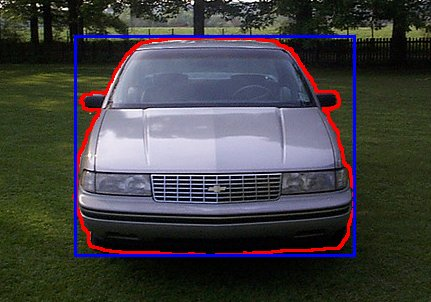
\includegraphics[width=0.4\textwidth]{images/shape-01}
\end{figure}

It is interesting to note that the above ratio does not depend on the size of
the image. Consequently, the discrimination based on this method ratio is
robust.

\subsubsection{Isoperimetric quotient}

Another ratio which can serve as a discriminator is the isoperimetric quotient.
The isoperimetric quotient is defined as the ratio of the curve area to the area
of a circle, \[\frac{4 \pi A}{p^2},\] where $A$ is the curve area and $p$ is the
perimeter of the curve \citep{isoperimetric-quotient:mathworld}. According to
the perimetric inequality, $4 \pi A \leq p^2$, the perimetric quotient never
exceeds 1 \citep{isoperimetric-inequality:springer}.

In other words, the isoperimetric quotient expresses the compactness of the
shape; the greater the quotient the more is the shape compact (the circle is the most
compact shape). When applied to a vehicle body, the resulting formula is \[
\beta = \frac{perimeter(H)}{area(H)} \] where $H$ is the corresponding hull
which is previously computed by the algorithm~\ref{algo:find-largest-hull}
described above, and functions $perimeter$ and $area$ calculate the perimeter
and the area of the hull, respectively.

The computation of the perimeter is trivial because of the fact that the
aforementioned algorithm ensures that all pixels which belong to the boundary
also belong to the hull. That being said, the perimeter can be defined as the
total number of hull pixels: \[perimeter(H) = |H|\]

To implement the computation of the isoperimetric quotient efficiently, a good
algorithm is essential. The naive approach would be to traverse all the pixels
which belong to a convex polygon $P_{convex}$ defined by the hull, and then
check for each such pixel whether it belongs to the hull $H$, which is not
necessarily convex. The time complexity of this method in Big-Oh notation is
$O(|H|^2)$, where $|H|$ is the number of pixels on the hull $H$. Not only does
the algorithm have the quadratic time complexity, but checking if a pixel
belongs to a non-convex polygon is also expensive.

Instead, an alternative approach is considered. Assume that pixels which belong
to the hull $H$ are partitioned into sets by their $y$-coordinate. Further, let
$X_y$ denote a sorted vector containing $x$-coordinates of all pixels which
belong to the corresponding partition, in ascending order. The indexing is
assumed to be 0-based. The area of the hull can now be computed as follows:

\begin{algorithm} 
\caption{Computes the area of the polygon defined by the hull}
\label{algo:hull-area}
\begin{algorithmic}
\REQUIRE $H$ is a valid hull consisting of adjacent pixels
\ENSURE $area$ is the area of the hull $H$, $area \geq 0$
\FORALL{$\left\{ y : (x, y) \in H \right\}$}
\FOR{$i \in [1, length(X_y) - 1]$}
\STATE $area \gets area + X_{y,i} - X_{y, i - 1}$
\ENDFOR
\ENDFOR
\RETURN $area$
\end{algorithmic}
\end{algorithm}

Consider a line $y = a$ which sweeps the image vertically, for each $a \in
[y_{min}, y_{max}]$, where $y_{min}$ and $y_{max}$ are the two extreme values of
y-coordinate on the hull $H$. Observe that, this way all pixels on the hull will
be scanned. Furthermore, since the hull is assumed to contain all pixels on the
boundary, it is guaranteed that every pixel which contributes to the overall
area is examined. Now, instead of examining every pixel along the line, it is
sufficient to determine two, as illustrated in figure
\ref{image:shape-area}.

\begin{figure}[htb]
\caption{Counting the number of pixels along the sweep line (shown in blue)
which belong to the area (shown in red).}
\label{image:shape-area}
\centering
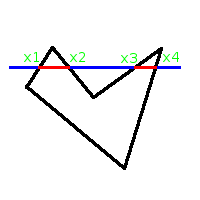
\includegraphics[width=0.4\textwidth]{images/shape-area}
\end{figure}

For instance, if $X_y = (x_1, x_2, x_3, x_4)$, the number of pixels with
$y$-coordinate equal to $y$ is $(x_2 - x_1) + (x_4 - x_3)$ (see figure
\ref{image:shape-area}).

The complexity of the above algorithm is $O(|H| \log |H|)$, where $|H|$ is the
number of pixels on the hull $H$. This is achieved by partitioning the pixels
first, which takes linear time, followed by sorting each partition.

\subsubsection{Side function median}

To compute the side functions, the hull points are first partitioned into
two disjoint sets, the set $L$ and $R$, based on whether they belong to the left
or right side, accordingly. The $x$-coordinate of the center of the hull's
bounding box, denoted as $x_{center}$ is set as the criterion for the
partitioning. Then, the side function of each side is computed as follows:
%%\[f_L(y) = \min{x : (x, y) \in L}\]
\[f_L(y) = \frac{\sum{\left\{x : (x, y) \in L\right\} }}
{|\left\{ x : (x, y) \in L\right\} |} - x_{center}\]
\[f_R(y) = x_{center} - \frac{\sum{\left\{x : (x, y) \in R\right\} }}
{|\left\{ x : (x, y) \in R\right\} |}.\]
Intuitively, these functions are defined as the average $x$-distance between the
horizontal line $x = x_{center}$ and every point at with the corresponding
$y$-coordinate.

The median of each of the two side functions is now simple the middle element of
the sorted vector obtained by taking the values for a side function and sorting
them.

\begin{algorithm} 
\caption{Partitions the hull points into two sets}
\label{algo:side-function-partition}
\begin{algorithmic}
\REQUIRE $H$ is a valid hull consisting of adjacent pixels
\ENSURE $L = \left\{ (x, y) : x < x_{th} \right\} \land 
R = \left\{ (x, y) : x > x_{th} \right\}$
\end{algorithmic}
\end{algorithm}

\begin{algorithm} 
\caption{Sorts a vector of points according to the y-coordinate, then
according to the x-coordinate if there is a tie}
\label{algo:sort-yx}
\begin{algorithmic}
\REQUIRE $V$ is the a vector of points
\ENSURE $\forall i \forall j (y_i < y_j \lor (y_i = y_j \land x_i \leq x_j))$
\end{algorithmic}
\end{algorithm}

\begin{algorithm} 
\caption{Computes the side function median of a set of hull points}
\label{algo:side-function}
\begin{algorithmic}
\REQUIRE $S$ is the set of points whose median $x$-coordinate is to be computed
\ENSURE $x_{median}$ is the median of the side function
\STATE $v \gets \begin{bmatrix}\,\end{bmatrix}$
\FOR{$(x, y) \in S$}
\STATE $v \gets \begin{bmatrix}v & (x, y)\end{bmatrix}$ \COMMENT{add point to
the vector}
\ENDFOR
\STATE $sort_{yx}(v)$
\RETURN $v_{|v| / 2}$
%%TODO
\end{algorithmic}
\end{algorithm}

\begin{algorithm} 
\caption{Computes the average side function median}
\label{algo:side-function-median}
\begin{algorithmic}
\REQUIRE $H$ is a valid hull consisting of adjacent pixels
\ENSURE $area$ is the area of the hull $H$, $area \geq 0$
\STATE $(x_{center}, y_{center}) \gets center(boundingbox(H))$
\STATE $(L, R) \gets sidepartition(x_{center})$
\RETURN $\frac{sidefunctionmedian(L) + sidefunctionmedian(R)}{2}$
%%TODO
\end{algorithmic}
\end{algorithm}

\subsection{Color discriminators}

The most notable discriminating feature of a vehicle is undoubtedly its color.
In spite of the fact that human visual system is very good at detecting and
identifying colors, as well as differentiating between them, this may be a hard
task for computers. This is due to the fact that the color of an object is
affected not only by the object itself, but also by various external factors.
These include nearby sources of light, such as from the public lighting or other
vehicles, as well as direct and ambient lighting from the sun or the sky.
Furthermore, since the vehicle bodies are glossy, it is easily possible that
light beams coming from the sky are reflected towards the camera; in this case,
the body acts as a mirror. The consequences are severe: a vehicle painted in
red, for instance, can suddenly become sky-blue or even yellow if sunbeams are
reflected directly.

There are two general approaches regarding color discrimination. The first one
is based on color classification; the two colors being compared are first
classified into groups and then it is checked whether both belong to the same
group. Unless some sophisticated techniques are used, such as locality-sensitive
hashing, this approach has similar disadvantages as the naive matching algorithm
from the previous section, where a thresholding method is applied; 
a minor classification error can have drastic consequences. The second approach tries to match the colors directly, without classifying
them first.

\subsubsection{The RGB color space}
It is a well-known fact that using three primary colors, red, blue and green, it
is possible to produce a broad array of colors by mixing them. Since the RGB
color model is additive, the intensities of these three colors determine the
secondary color; the higher the intensities, the brighter the secondary color.
For example, if the intensity of each color component is doubled, the intensity
of the resulting color is also doubled, but the hue remains unchanged. This
raises a question of how to differentiate the colors. Although one might try to
calculate the hue, or intensity for instance, from the intensities of the three
primary colors, this is discouraged because it makes the calculation
over-complicated; it is better to use other color spaces instead.

\subsubsection{The HSV color space}

The HSV color model solves some of the problems of the RGB color model,
especially when it comes to color (hue) perception. 

The figure \ref{fig:hsv-representation} shows the HSV color space. When moving
along circle, the hue changes, while the saturation and intensity remain
constant.

\begin{figure}[htb]
\caption{A common representation of the HSV color space}
\centering
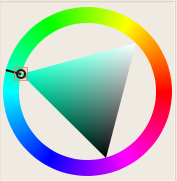
\includegraphics[width=0.25\textwidth]{images/hsv-representation}
\label{fig:hsv-representation}
\end{figure}


\subsubsection{Dominant features of a color}
At first glance, it seems that the color matching can be done using only the hue
component. However, that is not entirely true. When observing gray objects,
including white and black, it can be noticed that the variation in hue have
negligible effects on the visual perception of the color. The reason why gray
objects are not sensitive to the changes in hue lies in their saturation, i.e.
there is an absence of what we perceive as color.

Although not differentiable by the hue, the gray objects can be differentiated
by comparing their intensity in the HSV color space, which is, in fact logical.
A white object would have an intensity of $100\%$, while the black one would
have an intensity of $0\%$. That being said, the colors are divided into two
categories, the gray and the non-gray colors. As a criterion, the following method is
considered. If the saturation is high enough, the color should be represented
by the hue, since variations in hue greatly affect the perception of a
highly saturated color. Otherwise, the intensity should be considered, because
its variation, as said earlier, is what causes a certain object to be white,
black or somewhere in the middle, gray. 

When considering a thresholding method, one must also be aware that the
intensity also influences the color perception and thus the threshold itself. As
an example, in a dark room, although the saturation of the colors is high, the
intensity is low, and the differentiating power of color discrimination is
reduced to minimum. Having said that, the following thresholding method could be
used to determine the threshold in saturation, which dictates whether the
intensity or the hue of a color should be a dominant feature 
\citep{hsv:domimant-feature}.
\[ th_{sat}(V) = 1 - 0.8 V \]
In the formula above, the ranges of both intensity (denoted as $V$) and
saturation are assumed to be $[0, 1]$. It can be seen that for a low intensity,
the threshold approaches to $100\%$, since in a dark room only highly saturated
colors are differentiable, while in a bright environment the reverse is true.

\subsubsection{Vehicle body color extraction}
In order to be able to determine the color of a vehicle body and its dominating
features, the hull enclosing the body in the image needs to be found. Once the
hull is found, the pixels which belong to the region enclosed by the hull are
analyzed to eventually determine the color. An algorithm which finds the hull of
a vehicle body has already been described in the previous section.

The first thing which makes the task of color extraction complicated is various
parts of the vehicle which are either invisible, such as the windshield or
windows, or of a different color then the body, such as the wheels, the front
bumper etc. Because of these parts, if a color average of all pixels inside the
hull was computed, the result would probably be imprecise, especially if the
fact that windshield, which imitates the color of the vehicle interior, is
almost half the area of the body, when viewed from the front.

Therefore, a series of steps are required to isolate only the colored parts of
the vehicle, and these are definitely the hood (the region in the image between
the windshield and the front bumper or lights), and the roof (the region in the
image above the windshield). Since the color of the region between front lights
can be of a different color (usually black) from the rest of the body, to
simplify the segmentation of the hood, the front lights could be considered as
the boundary, instead of the bumper.

Surprisingly, the main part of the hood which is usually of the same color with
a simple algorithm. The algorithm calculates the y-coordinate of two horizontal
lines which enclose a region of the hood by calculating their relative positions
in the vehicle's bounding box. Because of the assumption that all images are
taken from the same angle, it is sufficient to multiply the height of the
bounding box with a constant. A similar heuristic algorithm can also be used to
extract the roof.

\begin{algorithm} 
\caption{Checks whether a pixel $(x, y)$ belongs to the hood region}
\label{algo:is-hood}
\begin{algorithmic}
\REQUIRE $bb$ is the bounding box of the region with the vehicle
\ENSURE $\top \iff (x, y)$ belongs to the hood region
\RETURN $hood_{min} \cdot height(bb) \leq y \leq hood_{max} \cdot height(bb)$
\end{algorithmic}
\end{algorithm}

\begin{algorithm} 
\caption{Checks whether a pixel $(x, y)$ belongs to the roof region}
\label{algo:is-roof}
\begin{algorithmic}
\REQUIRE $bb$ is the bounding box of the region with the vehicle
\ENSURE $\top \iff (x, y)$ belongs to the roof region
\RETURN $roof_{min} \cdot height(bb) \leq y \leq roof_{max} \cdot height(bb)$
\end{algorithmic}
\end{algorithm}

Finally, the two algorithms can be combined in order to obtain a simple
heuristic algorithm which can be used to filter the pixels with the aim of
removing the ones of which the color deviates from the body color.

\begin{algorithm} 
\caption{Checks whether a pixel $(x, y)$ belongs to the roof region}
\label{algo:is-bodycolor}
\begin{algorithmic}
\REQUIRE $bb$ is the bounding box of the region with the vehicle
\ENSURE $\top \iff (x, y)$ should be considered in calculating the body color
\RETURN $ishood(bb) \lor isroof(bb)$
\end{algorithmic}
\end{algorithm}

\subsubsection{Average color computation}
The average color of the body hull can now be simply computed. First, the pixels
are filtered with the $isbodycolor$ function, and then an average is computed.
Let $P$ denote the set of filtered pixels. If the RGB
color space is used, the computation of an average color is obtained by taking
the averages of each component (red, green and blue, respectively) and combining
the result. \[ avg_{RGB} = (\frac{\sum{r}}{|P|}, \frac{\sum{g}}{|P|},
\frac{\sum{b}}{|P|}), (r, g, b) \in toRGB(P) \] 
Here, the $toRGB$ function converts the
pixel position of each pixel from the input set to a triple $(r, g, b)$, which
denotes its color in the RGB color space, and returns the corresponding set.

\begin{algorithm} 
\caption{Checks whether a pixel $(x, y)$ belongs to the roof region}
\label{algo:find-body-pixels}
\begin{algorithmic}
\REQUIRE $H$ is the hull of the vehicle, $bb$ is the bounding
box of the image region with the vehicle
\ENSURE $P$ contains all pixels which should be considered in calculating the
body color
\STATE $P \gets \varnothing$
\FORALL {$(x, y) \in bb$}
\IF {$isbodycolor(x, y)$}
\STATE $P \gets P \cup (x, y)$
\ENDIF
\ENDFOR
\end{algorithmic}
\end{algorithm}


Once the average color is computed in the RGB color space, it is converted to
the HSV color space, which enables the dominating features, i.e. hue or
intensity, to be used as a discriminator.


\subsection{Licence plate discriminators}

Theoretically, the best discriminator is the vehicle's licence plate, since
vehicle licence place are unique in terms of the characters imprinted on them,
referred to as the licence plate number.

One possible, common, approach is to try to identify the licence plate
number for each vehicle. The image is first
filtered to boost contrast and reduce noise. Then, the characters are extracted
from the image. Finally, each character is recognized as a corresponding letter
or number using an artificial neural network. Reading the output of the neural
network for each character in the right order, the licence plate number is
obtained.

However, if a system is expected to correctly match licence plates anywhere on
the world, character recognition suddenly becomes a problem. One might try to
eliminate this problem by configuring the system for every country or region in
the world, but this is certainly a time consuming task, since it involves
obtaining a large collection of licence plate images. Even then, the system
would most likely be unable to match the vehicles from foreign countries or
regions, particularly if the visitor comes from a country where another alphabet
is used, such as the case with an arabic vehicle in a Western Europe
country, for instance.

For that reason, the SLESANN system does not even try to identify the licence
plate number. Instead, it tries to identify more general features of the
plate, which could also be the characters themselves.

\subsubsection{Filtering}

The first step towards feature extraction is image filtering. In this
system, licence plate image filtering consists of several phases. 

The first one is contrast enhancement. The goal of this phase is to separate the
color of the characters from the color of the background as much as possible.
For instance, if the characters are supposed to be black and the background is
supposed to be white, this phase should ensure that an image with moderately
brighter characters and darker background is converted to a black and white
image. Without boosting a contrast, an image of a licence plate captured in
dark, either at night or due to shadows, would be entirely dark, while an image
of the licence plate at direct sunlight would be all white. Another, even bigger
issue, is that all feature would need to be independent of the actual brightness
of the image, which is almost impossible in the case of vehicle licence plates.

In order to boost the contrast between the characters and the background, the
SLESANN system uses an algorithm called histogram equalization. The algorithm
originally works with grayscale images. Although the algorithm may
theoretically work on color images by applying it to the Red, Green and Blue components of the
RGB color values, this may yield dramatic changes in the image's color balance
since the relative distributions of the color channels change as a result of
applying the algorithm. Hence, the image is first converted to grayscale. After
that, histogram equalization algorithm is applied.

The second phase is noise elimination, as well as elimination of various
artifacts such as line borders of the plate, dirt stains, raindrops etc. Since
licence plates almost exclusively use two high-contrast colors, and these
artifacts worsen the plate discrimination, it is better to remove them. If this
phase was skipped, various discriminators based on characters in the plate would
be affected by these artifacts. For example, when a vehicle traverses a section
of a dirty road, its licence plates may become dirty, which means that two
images of the same licence plate may indeed have different features. The similar
effect happens in the case of a sudden rain.

To eliminate the aforementioned artifacts, the following trick will be used.
Since they are usually much smaller then the characters themselves, an
appropriate algorithm has to be chosen. Under the assumption that the background
is white, which can be simply assured, the algorithm works as follows. For each
pixel $(x, y)$, a square of side length equal to $2 d$ around the pixel is considered. Then, the average color inside
that square, denoted as $T(x, y)$ is computed. Now, the value is compared
against it; if it is greater then the threshold decreased by some constant,
denoted as $C$, the pixel color should be totally black. Otherwise, the pixel
should be totally white. If the intensity is represented as a real number from
range [0, 1] the following function determines the new color of the pixel.
\begin{displaymath}
   color'(x, y) = \left\{
     \begin{array}{lr}
       1, & color(x, y) > T(x, y) - C \\
       0, & color(x, y) \leq T(x, y) - C
     \end{array}
   \right.
\end{displaymath}
The above method is known as adaptive thresholding because it uses a dynamic
threshold based on the neighborhood of the pixel to which it is applied, as
seen from the function above.

%Since the aforementioned artifacts are usually much smaller then the characters
%themselves,  The actual algorithm used for artifact removal is the
%above-mentioned artifacts is

The last phase of the image filtering is character extraction. In this phase,
the character are not recognized nor identified, but only extracted. In other
words, the characters are treated as black connected components. Thus, the first
step in this phase is running the well-known connected components algorithm. 

In graph theory, the problem of finding connected components is most commonly
solved with the flood-fill algorithm in linear time, proportional to the number
of vertices in the graph. Although the same approach could be used for finding
connected components in the image, its use is discouraged because there exists
another algorithm. This algorithm, known as the two-pass algorithm, has the same
time complexity, but runs faster since it finds all connected components in a
two-dimensional binary image in exactly two passes \citep{two-pass-algorithm}.

Once the black components are found in the binary image, they are sorted in
descending order by their size. The size of the component is defined as the
number of pixels in the component. To extract the characters, it is sufficient
to take the right number of largest components. Lastly, based on components'
sizes, it is possible to apply further filtering with the aim of removing small
artifacts which ``survived'' the previous filters.

\begin{figure}[htb]
\caption{The artifact removal steps on a plate with a large
artifact in the top-right corner}
\centering
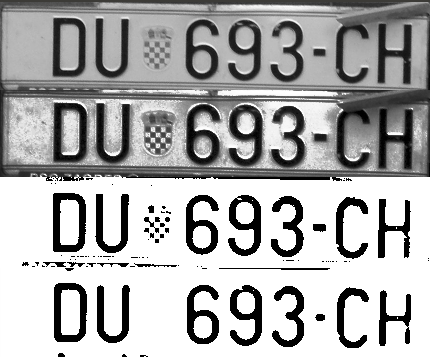
\includegraphics[width=0.5\textwidth]{images/artifact-removal-01}
\label{fig:artifact-removal-01}
\end{figure}

\begin{figure}[htb]
\caption{Artifact removal steps on a plate full of
dirt stains}
\centering
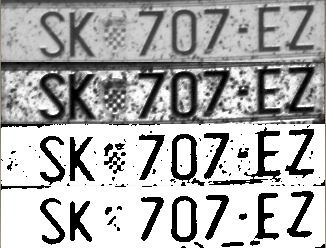
\includegraphics[width=0.5\textwidth]{images/artifact-removal-02}
\label{fig:artifact-removal-02}
\end{figure}

The figures \ref{fig:artifact-removal-01} and \ref{fig:artifact-removal-02} show
artifact removal steps. From top to bottom:
\begin{enumerate}
  \item grayscale image of the plate
  \item image after histogram equalization is applied
  \item binary image after one iteration of adaptive thresholding
  \item binary image after several iterations of adaptive thresholding
  with smaller values of parameter $d$
\end{enumerate}

\begin{figure}[htb]
\caption{Filtering process on two images of the same licence plate}
\centering
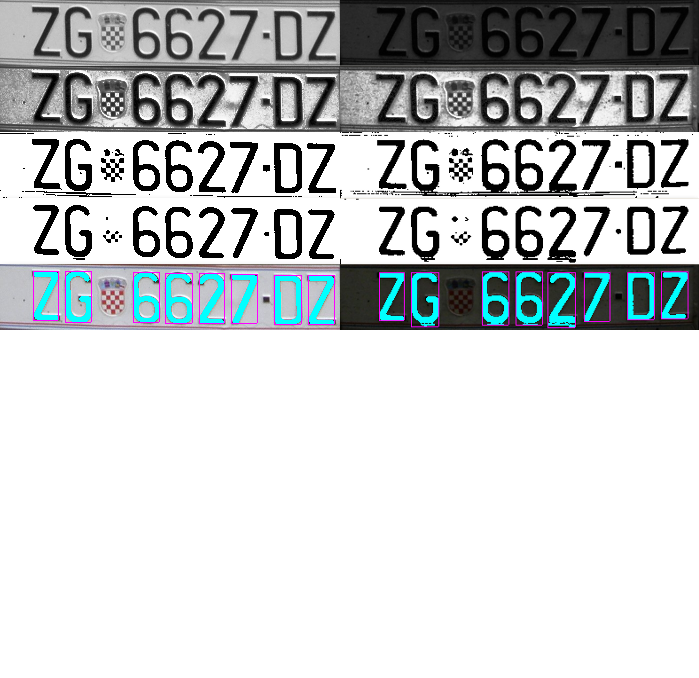
\includegraphics[width=0.85\textwidth]{images/filter-all-scaled}
\label{fig:plate-filter-all}
\end{figure}

The figure \ref{fig:plate-filter-all} shows the whole filtering process applied
to two different images of the same licence plate. It is visible that the
filtering algorithm, as well as character extraction algorithm, both produce
good result, even though the intensities and contrasts of initial images are
entirely different.

\subsubsection{Portion of black pixels}

One of the simplest matching discriminator of a binary image is the portion of
black pixels in the image. Assuming the pixel values are either 0 or 1, as
before, the portion of black pixels is equivalent to the average color of the
image, \[ \frac{\sum_{1 \leq x \leq w, 1 \leq y \leq h}{color(x, y)}}{w h} \]

The discriminating power of this value is limited, but it should still be able
to differentiate the two licence plate images with varying number of
characters.

\subsubsection{Normalized vertical/horizontal projection}

Another common feature used in image analysis is vertical/horizontal
projection. These projections are calculated by computing the sum of pixel
color values in each column/row of the image. This way a vector is obtained,
which can be treated as a function.

There is one problem with this approach when applied to vehicle plate
discrimination. To make vertical and horizontal projections of the two images
comparable, both images would need to be scaled to the same resolution, since
the upper bound of the sums of the columns/rows is proportionate to the image
height/width. Nevertheless, the SLESANN system avoids scaling the licence plate
images to the same size. Since licence plate regions are relatively small
compared to the size of the vehicle in the image, any scaling would have an
impact on image quality and, consequently, the features that could be extracted
themselves. Yet another problem with scaling is that the aspect ratio of the
plalte is not preserved since the dimensions of licence plates vary, not only
depending on the vehicle type (e.g. motorbikes, trucks etc.), but also the
country/region.

However, only two changes are necessary to ``normalize'' the projections, so
that they are mutually comparable. First, a vertical/horizontal projection is
divided by the height/width of the image, which is equivalent again equivalent
to taking the average instead of the sum. In the case of binary images, provided
that the pixel color values are either 0 or 1, the average of a column/row is
actually equivalent to the portion of black pixels in it. Second, instead of
taking the average in each column/row, the average of several columns/rows is
being computed. More precisely, when vertical projection is computed, the image
is split into a fixed number of rectangles of the approximately same width,
formed by merging the adjacent columns together, and these rectangles are then
treated as columns. The analogous trick is used to compute normalized horizontal
projection.

In order to extract the most information out of the image, we need to determine
the optimal number of rectangles to divide the image into, which is equivalent
to the size of the normalized vertical projection vector. Let $N$ denote that
number. Observe that for $N = 1$, the vertical projection is equal to the
portion of black pixels in the image. On the other hand, making $N$ large, for
example $N = w / 2$, the values of the normalized projection vector are very
sensitive to image translation or even slight variation in viewing angle. Thus,
the optimal value for $N$ should be somewhere in the middle. 

It makes sense, however, to consider the multiples of $N$, especially the small
ones. For instance, if $N$ is equal to average number of characters on the
licence plate, it is reasonable to expect that some of the letters will
completely fall into one of the rectangles. For other multiples of $N$, the
similar effect is produced, with the difference that only part of a character
falls into a rectangle. Because of this, the normalized projection vector of the
size which is a small multiple of $N$ looks like a promising discriminator. This
discriminator is also more robust than any discriminator based on the connected
components, since this one does not rely on the number of characters or the
connectivity of the black pixels in the image.

\subsubsection{Components' normalized centroids}

The components' centroid is another possibly good discriminator. For example,
the characters 'J' and 'L' have diametrically opposed centroids when comparing
the centroids' x-coordinate. The centroid is here defined as the average
position of black pixels. In order to ensure that centroids of two components
can be compared, they are normalized in the following way:
\[ c_{norm} = (\frac{c_x - x_{min}}{width(bb)}, \frac{c_y -
y_{min}}{height(bb)}), \]
where $c_x$ an $c_y$ denote a centroid, $bb$ represents the components'
bounding box and the points $(x_{min}, y_{min})$ is the upper left corner of the
bounding box.

\section{Match probability computation}
Once the various matching discriminators are obtained, they can be used as
inputs in one or more ANNs. 

When observing vehicles, it can be noticed that the color of a vehicle rarely
determines its shape and vice-versa. For example, if a vehicle is blue, this
does not mean that it is manufactured by a specific manufacturer. Similarly, the
vehicle manufacturer rarely paint their vehicles in unique colors. It is also
true that the correlation between the vehicle licence plate number and the
vehicle manufacturer, and thus the shape, is negligible.

This observation enables the matching probability of the two images to be
computed independently, with respect to shape and color discriminators and the
features extracted from the vehicle licence plate. The main reason to split the
matching process into three sub-processes is to reduce the size of the ANNs used
to compute the matching probabilities.

Once the matching probability is computed based on the vehicle shape, color and
its licence plate, another neural network can, although need not be used,
to determine the total matching probability based on these three matching
probabilities.

\subsection{Cache}

In section \ref{section:matching-algorithm}, where the matching problem of
matching the images from sets $L$ and $R$ was described and analyzed, one
important detail was omitted, and that is the computation of the probability
matrix $p$.

Since the ANNs required discriminator values of the two images to be computed,
the question is whether to compute them whenever they are needed by an ANN, or
to cache the already computed discriminator values so that the discriminator
values obtained from the same image are not computed multiple times. Without
loss of generality, assume that $|L| = |R|$. In the case of the former,
discriminator values of each image is computed exactly $|L|$ times, which
results in a total of $|L|^2$ discriminator values computations. In case of the
latter, however, the discriminator values of each image is computed only once,
thus resulting the total of $|L|$ computations, with the limitation that only
discriminator values which depend on a single image can be cached.

As seen from the previous sections, none of the discriminators are based on
extracting features from two images simultaneously. Furthermore, considering the
fact that matching discriminators are actually one or at most few real numbers,
it is evident that caching can be performed with a reasonable amount of
memory used.

\subsection{Artifical neural network}

\subsubsection{Input and output transformation}

If a sygmoidal activation function is used, which is a common choice when it
comes to ANNs, the inputs and outputs need to be scaled to the interval $[-1,
1]$. The probability can be simply scaled by multiplying it by 2 and the
subtract 1 from the product, thus
\[i = 2 p - 1 .\]
As regards input, since the majority of matching discriminator are already
normalized to interval $[0, 1]$, the same formula from above applies.
Discriminators such as the hue average are transformed in a similar way. 

\subsubsection{Training the network}

In order to be able to compute the probability, the ANNs must be trained first.
The training consists of a series of inputs and outputs. Since the ANN in this
particular system is supposed to compute the matching probabilities of the given
two images, it should be trained accordingly. The training consists of a series
of data sets in which the discriminator values of the two images are used as
inputs, and the scaled probability is used as the expected output. 
During the training phase, the network iteratively adjusts the weights between
connected neurons in a number of steps, with the aim of minimizing the average
sum of the differences between expected outputs and actual outputs. This
average is known as mean square error.

When creating a training data set, it is hard to guess the exact, or near-exact,
matching probability of the the images. Therefore, the simplified approach is
considered; if the images match the expected probability is set to 1, otherwise
it is set to 0. Assuming the sygmoidal activation function is used, this means
that the outputs in the training data set are $-1$s or $1$s. The
same applies to the data set used for testing the neural network.
Since the weights of the neuron connections in the artificial neural networks
are real, this does not prevent the network itself to express its own certainty,
or in other words ``probability'' that the two images match.

\subsubsection{Testing the network}
It is recommended that a separate data set is used to test a neural network.
This way, it is easy to check whether a network has been overfit during the
training phase. Overfitting has a loss of generalization as a consequence,
which means that such a network is too adapted to the data set used for training
and produces a relatively big mean square error when a previously unseen test
data set is used.

\subsubsection{Using the network}
Once the network is trained, it can be saved to a file, for instance, and then
used multiple times, whenever a matching probability of two images needs to be
computed. The caching can be used to avoid computation of the discriminator
values of the same image twice.

\chapter{Software implementation}

\section{Programming languages}
A real-time system which is expected to work in almost any situation needs to be
both efficient (in terms of energy consumption) and fast (in terms of
computational speed).
 
Another thing that is to be taken into consideration is portability, i.e. the
ability that the application can be run on embedded hardware, possibly with
different operating system. For instance, a system which is able to operate with
embedded computers which process the data captured by a camera could result in
significant cost reduction as regards energy consumption.

The C++ programming language was chosen as the main programming language for a
reason; it is generally portable (provided that the libraries used are portable
as well) and its speed is comparable with C, one of the fastest compiled
programming languages.

Apart from C++, since the project required a lot of file system operations, such
as copying, moving and classifying images, and tampering with files and other
data, BASH was used as a glue language. Several scripts have been written in
BASH, which mainly aim to automate the process of preparing input data for
artificial neural networks used in the project.

\section{Development environment}
Throughout the project, the platform used was Ubuntu Linux 10.04, with GCC (GNU
Compiler Collection) 4.4.3 C++ compiler. The IDE used for development was
Eclipse (version Helios).

As a part of this thesis, a software application has been written in the C++
programming language. The application consists of a set of independent modules,
totaling over 10000 lines of code.

\section{Libraries}
\subsection{Boost}
Apart from its popularity, the quote ``..highly regarded and expertly designed
C++ library projects in the world'' from a popular book on C++ programming was
another reason to use Boost C++ libraries
\citep{boost:quote-c++-coding-standards}. The following libraries from the
collection have been used throughout the project:

\subsubsection{Filesystem}
The C++ Standard Library does not provide a portable implementation for file
manipulation, therefore the Boost.Filesystem library was used instead. This way,
not only the application remained portable, but it was also easy to do common
operations such as file creation, copying, moving or checking if a file or
directory exists etc.

\subsubsection{Smart Ptr}
The use of smart pointers in a programming project of this size can
significantly simplify the development, while also preventing memory leaks. The
Boost.SmartPtr library has done its job very well in the sections of code where
the need of automatic memory management was needed.

\subsubsection{Date Time}
The SLESANN, just as any other real-time system, requires a lot of manipulations
on timestamps. Therefore, an appropriate time library was needed. Again, as the
C++ Standard Library does not provide a portable implementation for this
purpose, an alternative had to be chosen. Boost.DateTime seemed like a perfect
choice, both because of its popularity and the fact that adding one more of the
Boost libraries would not increase the overhead.

\subsubsection{Units}
Although, at first glance it might seem unnecessary to include just another
library from Boost collection, a sophisticated, type-safe implementation of unit
systems, with plenty of conversion methods was used. This library enables the
system to be implemented in various regions of the world with almost no changes
to the code needed - it is sufficient to write a module which handles the input
differently and calls the appropriate conversion functions from the library.

\subsubsection{Program Options}
This library enabled an easy, yet portable way of processing command line
arguments.

\subsection{OpenCV}
Since the project involves a significant amount of image processing, most of
which occurs in real time, a good library was a necessary tool. Being both
open-source and cross-platform, with more than 2 million downloads, OpenCV has
proven to be the right choice \citep{opencv-wiki:main}.

The version used for this project was 2.1, primarily because of its new C++
interface and the fact that official documentation for version 2.2 has not yet
been released.

\subsection{Fast Artificial Neural Network Library (FANN)}
Being fast and easy to use and well-documented, the
FANN Library was proven to be a good choice as
regards artificial neural networks \citep{fann:sf-summary}. 

\subsection{Google C++ Testing Framework}

This testing framework has been chosen for several reasons. First of all, it is
cross-platform. Second, it has automatic test discovery, so there is no need to
register every single test unit. Finally, it has the rich set of assertions
\citep{gtest:gcode-summary}. Some of the assertion methods, such as floating
point number comparison with a given tolerance, proved to be very convenient in
component testing. The built-in timer helped boost performance of performance
critical code sections of the project.

\subsection{libhungarian}

Libhungarian is a small C-library which implements the Hungarian algorithm. This
is actually a slightly enhanced version of the implementation provided by the
Stanford GraphBase \citep{libhungarian:stachnis}. This algorithm, and the
library itself, is used in the core matching module of the project to provide
well-tested code.

The source code inside \texttt{src/matching} is written as a bridge to the rest
of the project. This allows the rest of the project to be independent of the
libhungarian library, which resides in the \texttt{src/matching/libhungarian}
directory.

\subsection{EZtester}
This small logging library was used for convenience, to avoid writing one from
scratch. Although Boost has its own logging library, this one seemed like
more appropriate because of its simplicity and the fact that there was no need
for such a sophisticated logging mechanism provided by Boost.Log.

Although the library itself is supposed to be cross-platform, in order to work
with GCC 4.4.3 compiler (on Ubuntu Linux 10.04), some minor changes have been
done to the original implementation. 

\nocite{ezlogger:overview}

\chapter{Experimental results}

\section{Image acquisition and preparation}

In order to test some parts of the SLESANN system, a moderately large set of
images needed to be obtained. Although there may exists some public databases
with vehicle images, in order to obtain the best image for testing, it was
decided to do a multiple session shooting at a public parking lot with a
reasonable number of parked vehicles.

The decision not not use images of the moving vehicles, which the SLESANN system
usually work with, was made for two reasons. First, it is relatively hard to
obtain blurless images with a non-stationary, non-professional camera. Second,
the only significant difference in the image is the absence of a driver or other
persons in the vehicle. The latter, however, does not play any significant role
because none of the described methods use the windshield part of the image.

\subsection{Image acquisition}

The collection consists of 161 photographs of vehicles at the public parking lot
situated between Babićev prilaz and Radauševa streets in Zagreb, Croatia. There
were five shooting sessions, at different times of the day, including days
when the weather was sunny, clear, cloudy etc. Although lighting conditions
vary from photograph to photograph, all photographs were taken during daylight
to ensure the validity of test data for matching (it is impossible that a
vehicle passes first checkpoint at day but second at night). The alternative
would be to classify the images into two groups, i.e. day and night images, and
test matching on each of the group separately.

All photographs were captured with Olympus SP-560 UZ digital camera, at 3264
$\times$ 2448 resolution. The resolution was then scaled down to 50\%, to reduce
image processing time, as well as transfer times during testing. The photographs
are stored as JPEG images.

The photographs were captured from a standing position, from the approximately
same distance and angle. The latter is of the utmost importance, because the
angle affects the shape of a vehicle body. The former may also result in slight
deformations of the shape and is therefore taken into consideration during
shooting.

\subsubsection{Image diversity}
Since the photographs are to be used for matching purposes, there was a tendency
to capture images of the same vehicles as many times as possible, while still
keeping the diversity of the vehicles. If only two images of each vehicle were
captured instead, it would not be possible to generate the sufficient number of
positive test cases where the images actually match, since those two numbers are
quadratically proportional. 

% % frequencies {2: 15, 3: 8, 4: 3, 5: 3, 6: 1, 7: 1}

\subsection{Vehicle image segmentation}
To be able to extract shape, color and plate discriminating features from
vehicle images, the segmentation must be done first.

\subsubsection{Body segmentation}

The existing methods for segmentation, are subject to various types of errors
and imprecision. For example, a code book segmentation can be tricked when two
moving vehicles are in the same image. Thus, to avoid errors caused by
segmentation and improve the quality of measurements, it is decided to do the
segmentation manually.

The image processor program used was GIMP v2.6, and a BASH script called
\texttt{extract-bodies.sh} which automated some the process of manual
segmentation, a total of 143 images were obtained. When compared to the total
number of images, it can be seen that exactly 19 of them are missing; this is
because those were taken from wrong angles, have an obstacle like tree branches
etc., or some part of the body which affects shape is not visible.


\subsubsection{Plate segmentation}
The problem of vehicle licence plate segmentation is even harder than vehicle
body segmentation. Therefore, plate segmentation was done manually as well.
Again, another BASH script, \texttt{extract-bodies.sh} was used to automate
image editing in GIMP. A total of 161 images is obtained in this way.

\section{Feature evaluation}

Once the body and licence plate are segmented, they can be used to extract
various features describing them. As a part of the experimental work, all of the
features described in section \ref{section:matching-discriminators} were
implemented, tested and analyzed.

Now, the key problem is to determine which features are good discriminators and
are as such worth being a part of the input to an artificial neural network.

From the statistical point of view, a good feature might be the one whose values
do not vary much inside the same group, but varies much outside the group. The
former is measured by comparing values of the feature for each image which
belongs to the group, while the latter is measured by comparing the average
value of the group to the averages of other groups.

Formally, the evaluation of goodness of a particular feature is defined as \[
\eta = \frac{1}{|G|} \cdot \sum_{i \in G}{\frac{\sigma_{i}} {\frac{1}{|G| - 1}
\cdot {\sigma_{G \setminus i}} }}. \]

To simplify the calculation, two changes can be made to the above formula.
First, the standard deviation of each group can be approximated with the average
standard deviation of the samples of the same group. Second, the standard
deviation of the average values of other groups can be approximated with the
average. This results in the following formula: \[\eta =
\frac{\sigma_{same}}{\sigma_{other}}, \] where $\sigma_{same}$ is the average
standard deviation of the values inside a group and $\sigma_{other}$ is average
the standard deviation of the averages of the other groups.

\subsection{Shape discrimination}

In order to evaluate the goodness of each shape discriminator as precisely as
possible, the images of vehicles were first sorted by manufacturer. Then, each
pair of images of a vehicle of the same manufacturer is compared manually to
check if the same vehicle model is in both images. If so, they are grouped
together. The obtained group distribution is shown in figure
\ref{fig:shape-group-distribution}.

\begin{figure}[htb]
\centering
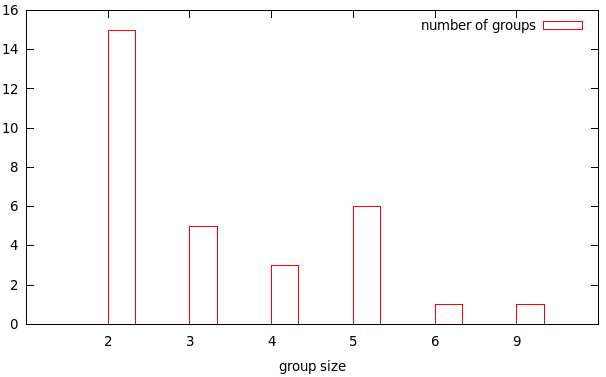
\includegraphics[width=0.85\textwidth]{images/shape-group-distribution}
\caption{Distribution of groups used for shape discrimination evaluation}
\label{fig:shape-group-distribution}
\end{figure}

%\begin{table}[h]
%\begin{center} {\footnotesize
%\begin{tabular}{c|c|c}
%\# group & number of images in the group \\
%\hline
%1 & 2 \\
%\end{tabular} }
%\end{center}
%\caption{\footnotesize Number of turns and distance between top and bottom.}
%\label{turns}
%\end{table}

Finally, the goodness of each shape discriminator is evaluated as described
above. The results are shown in table
\ref{table:shape-discriminators-goodnesses}.

\begin{table}[h]
\begin{center} {\footnotesize
\begin{tabular}{c|c}
Matching discriminator name & goodness
($\frac{\sigma_{same}}{\sigma_{other}}$) \\
\hline
isoperimetric quotient          &                    3.6047 \\
height / perimeter              &                    3.1519 \\
width / perimeter               &                    2.2976 \\
side function median            &                    2.1300 \\
normalized height               &                    2.0044 \\
side function average           &                    1.8521 \\
width / height                  &                    1.9933 \\
rectangularity                  &                    1.5259 \\
\end{tabular} }
\end{center}
\caption{\footnotesize Goodness values of shape discriminators, sorted in
descending order}
\label{table:shape-discriminators-goodnesses}
\end{table}

Comparing goodness values of the discriminators listed in the table above, it 
can be noted that there is a large gap in goodness value between the second and
the third row. This can be interpreted as the fact that the
shape discriminating power of perimeter quotient and height-perimeter quotient
is good, at least compared to other shape discriminators.

It can also be observed that the standard deviation of the median over samples
of the same shape was less than the standard deviation of the average function. For
that reason, the median was chosen instead of the average to be used as one of
the inputs for the corresponding artificial neural network.


\subsection{Color discrimination}

As regards color, there is always a dilemma whether or not two red vehicles, for
instance, are exactly of the same color, or not. It is sometimes different to
guess the color correctly, especially if various changes in lighting conditions
are considered. Therefore, when creating color groups, certain care was taken;
only strongly differentiable color groups were considered. This means that
similar color groups, like the ones containing images of dark-blue and navy blue
vehicles are mutually exclusive. This groups are not simultaneously present in
the same data set.

In the decision of which of the mutually exclusive groups to include into the
test case, larger groups were preferred, primarily because they actually
represent the most common colors, including black, white, gray, blue, red and
some fade colors like cyan, light brown etc. A test case consisting of 75
images of the vehicles of 8 different colors is obtained.

\begin{figure}[htb]
\centering
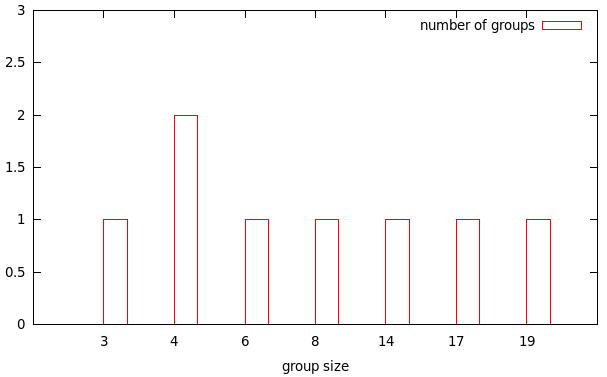
\includegraphics[width=0.85\textwidth]{images/color-group-distribution}
\label{fig:color-group-distribution}
\caption{Distribution of groups used for color discrimination evaluation}
\end{figure}

Using these color groups, the following results for goodness evaluation are
obtained.

\begin{table}[h]
\begin{center} {\footnotesize
\begin{tabular}{c|c}
Matching discriminator name & goodness
($\frac{\sigma_{same}}{\sigma_{other}}$) \\
\hline
portion of hue-dominant pixels                   &    7.4102 \\
average saturation                               &    3.4415 \\
average saturation from dominant pixels          &    2.8397 \\
hue least square fit of hue-dominant pixels      &    1.8436 \\
average hue                                      &    1.7318 \\
average intensity                                &    1.3174 \\
average intensity of intensity-dominant pixels   &    1.3115 \\                 
\end{tabular} }
\end{center}
\caption{\footnotesize Goodness values of color discriminators, sorted in
descending order}
\label{table:color-discriminators-goodnesses}
\end{table}

The results illustrate the importance of saturation value in when discriminated.
Not only is it the second-best of the above discriminators, but its consequences
are even bigger; as already explained in section
\ref{section:matching-discriminators}, the saturation value can be used to
define a threshold for determining whether to represent a pixel by hue or
intensity. That is an explanation why the portion of hue-dominant
pixel has such a high goodness value.

\subsection{Licence plate discrimination}

In case of plate discrimination, the groups for evaluating goodness values are
simple to construct since they correspond to the actual licence plate numbers in
the images. The distribution is shown in figure
\ref{fig:plate-group-distribution}. In order to decide how many discriminators
and which among them to consider, it was first necessary to determine the
optimal value for parameter $N$ which is used to calculate normalized vertical
projections.

\begin{figure}[htb]
\centering
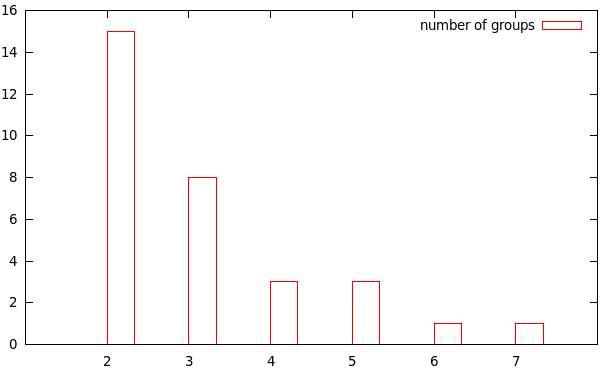
\includegraphics[width=0.85\textwidth]{images/plate-group-distribution}
\label{fig:plate-group-distribution}
\caption{Distribution of groups used for plate discrimination evaluation}
\end{figure}

The experimental results shown in figure \ref{fig:ver-proj-lsf} confirm
the previous suspicion that the parameter $N$ should be close to a multiple of
the number of the number of characters on the plate.

\begin{figure}[htb]
\caption{Least square goodness value fitting of normalized vertical projection}
\centering
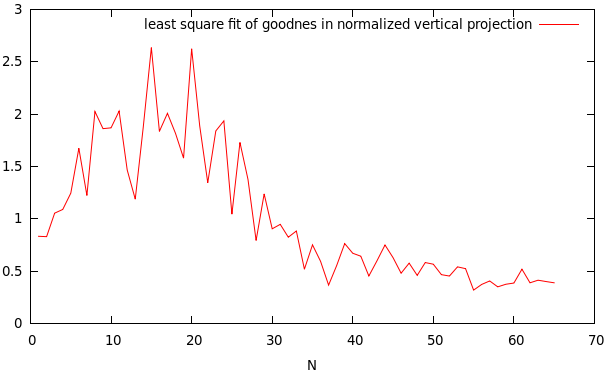
\includegraphics[width=0.85\textwidth]{images/ver-proj-lsf}
\label{fig:ver-proj-lsf}
\end{figure}

As visible from the graph in figure \ref{fig:ver-proj-lsf}, the part of the
function between 8 and 10 looks promising, so $N$ was chosen to be equal to 8.
This means that eight regions of plate are considered and for each region the
portion of black pixel is computed, which is equivalent to the computation of
normalized vertical projection with $N = 8$. For the similar reason, the number
of character for which the normalized centroid is computed is also equal to 8.  

Finally, the following are results of goodness evaluation for plate
discriminators.

\begin{table}[!ht]
\begin{center} {\footnotesize
\begin{tabular}{c|c}
Matching discriminator name & goodness
($\frac{\sigma_{same}}{\sigma_{other}}$) \\
\hline
rectangularity, component 1                     &    1.6225 \\ 
rectangularity, component 2                     &    1.1737 \\ 
rectangularity, component 3                     &    3.3581 \\ 
rectangularity, component 4                     &    1.5692 \\ 
rectangularity, component 5                     &    2.2993 \\ 
rectangularity, component 6                     &    2.3115 \\ 
rectangularity, component 7                     &    1.2767 \\ 
rectangularity, component 8                     &    2.1192 \\ 
$c_{norm, 1, x}$                                &    1.7628 \\ 
$c_{norm, 2, x}$                                &    1.0133 \\ 
$c_{norm, 3, x}$                                &    2.3836 \\ 
$c_{norm, 4, x}$                                &    3.2315 \\ 
$c_{norm, 5, x}$                                &    1.7898 \\
$c_{norm, 6, x}$                                &    1.3299 \\
$c_{norm, 7, x}$                                &    1.1953 \\
$c_{norm, 8, x}$                                &    1.8572 \\
$c_{norm, 1, y}$                                &    1.1002 \\
$c_{norm, 2, y}$                                &    1.0916 \\
$c_{norm, 3, y}$                                &    2.4817 \\
$c_{norm, 4, y}$                                &    1.7131 \\
$c_{norm, 5, y}$                                &    1.8387 \\
$c_{norm, 6, y}$                                &    1.7949 \\
$c_{norm, 7, y}$                                &    1.5556 \\
$c_{norm, 8, y}$                                &    1.9449 \\
black pixel portion, region 1                   &    0.9581 \\ 
black pixel portion, region 2                   &    0.9883 \\ 
black pixel portion, region 3                   &    1.1269 \\ 
black pixel portion, region 4                   &    1.9884 \\ 
black pixel portion, region 5                   &    1.2582 \\ 
black pixel portion, region 6                   &    1.9651 \\ 
black pixel portion, region 7                   &    1.3771 \\ 
black pixel portion, region 8                   &    1.1373 \\
\end{tabular} }
\end{center}
\caption{\footnotesize Goodness values of plate discriminators}
\label{table :color-discriminators-goodnesses}
\end{table}

\section{Matching probability computation}

The aim of goodness values computation in the previous section was to check
whether a certain discriminator has enough discriminating power. Now, the
discriminators which are good enough are used to compute input vectors for ANNs.

In order to build training data sets for the artificial neural networks, as well
as data sets used for validation, the same groups used for goodness evaluation
are used. However, since two separate sets are to be built, approximately half
of the images from each group were included in each data set, resulting in two
data sets with parts of the original groups preserved (i.e. none of the
groups in the two data sets includes images originating from multiple initial
groups).

The expected outputs are computed by checking the groups of the two images used
to build the corresponding input vector; if both image belong to the same group,
this means that they match when considering only the color, the shape or the
licence plate. The values $1$ and $-1$ are used to indicate whether the two
images match or not, respectively.

The question is now, whether the number of positive and negative outputs should
be balanced. The experiments showed that if this is not the case, the network
becomes biased in a way that it tends to produce the output which is dominant
most of the time. For instance, if 95\% of the outputs are negative, since the
network tries to minimize the mean square error, it easily achieves this by
adjusting the weights so that output is always negative; this ensures a relative
mean square error of 5\%, which is hard to beat unless the test data is very
consistent.

The training data was generated with a script which first builds all
possible input vectors and then removes some of the test data in order to
achieve the balance between the number of input-output pairs with positive and
negative output.

To evaluate the results of matching probability computation, the following two
parameters are measured during the training.

\begin{enumerate}
  \item Mean square error, $\sum_{i}{(o_{expected} - o_{actual})^2}$
  \item Bit fail count, defined as the total number of wrong outputs where the
  actual output is more than 35\% incorrect %\[ \sum_{i}{ \sgn{ 
     %\frac{  \abs{o_{expected} - o_{actual}} } {0.7} 
   % } }
  %\] %%TODO
\end{enumerate}

Since there is only one output neuron in each network, and the probability is
measured, the bit fail count is equivalent to the number of test cases for which
the expected and the actual probabilities differ by more than 0.35. That being
said, the reliability of the network can be expressed as \[ \rho = 1
- \frac{b}{N}, \] where $b$ is the bit fail count and $N$ is the size of the
test data, determined by the number of test cases contained within it.

\subsection{Shape matching probability}

The properties of data sets used to train and test the artificial neural network
for computing shape matching probability are shown in figure 
\ref{table:shape-data-properties}.

\begin{table}[h]
\begin{center} {\footnotesize
\begin{tabular}{c|c|c|c|c|c}
Data set & groups & different images & positive & negative & positive (\%) \\
\hline
Train & 24 & 47 & 198 & 198 & 0.5 \\
Test & 7 & 28 & 120 & 120 & 0.5 \\
\end{tabular} }
\end{center}
\caption{\footnotesize Properties of training and test data set for color
discrimination}
\label{table:shape-data-properties}
\end{table}

Figures \ref{fig:shape-train-01-bf}, \ref{fig:shape-train-01-mse},
\ref{fig:shape-train-02-bf} and \ref{fig:shape-train-02-mse} show the training
performance of the network when varying different parameters, including the
number of neurons in each layer, the training algorithm used, as well as other parameters such as
learning rate. 

The precise results are shown in table \ref{table:shape-training-results}. By
looking at reliabilities, denoted as $\rho$, it can be seen that the reliability
is good for training data set, but bad for test data set. While the probability
of the correct computation of matching probability of two images from the
training set is above $0.95$, the probability of computing the shape matching
probability incorrectly for two previously unseen images is around $0.5$.

\begin{table}[h]
\begin{center} {\footnotesize
\begin{tabular}{|c|c|c||c|c|c||c|c|c|}
\hline
\multicolumn{3}{|c||}{network description} & 
\multicolumn{3}{c||}{training data set} & 
\multicolumn{3}{c|}{testing data set} \\
\hline
neurons & training & learning & MSE & $b$ & $\rho$ & MSE & $b$ & $\rho$ \\ 
by layer & algorithm & rate    & & & & & & \\
\hline

10-4-1 & RPROP & - & 
0.0203196 & 10 & 0.975 & 
0.501151 & 120 & 0.500 \\

10-2-1 & Incremental & 0.5 & 
0.0336083 & 19 & 0.952 & 
0.500688 & 120 & 0.500 \\

10-10-5-2-1 & RPROP & - & 
0.0295715 & 12 & 0.970 & 
0.503730 & 120 & 0.500 \\

10-20-10-5-1 & RPROP & - & 
0.0109151 & 4 & 0.990 & 
0.533576 & 128 & 0.467 \\

\hline
\end{tabular} }
\end{center}
\caption{\footnotesize Properties of training and test data set for shape
discrimination}
\label{table:shape-training-results}
\end{table}


\begin{figure}[htb]
\caption{Mean square error through epochs of incremental and RPROP training
for shape matching}
\centering
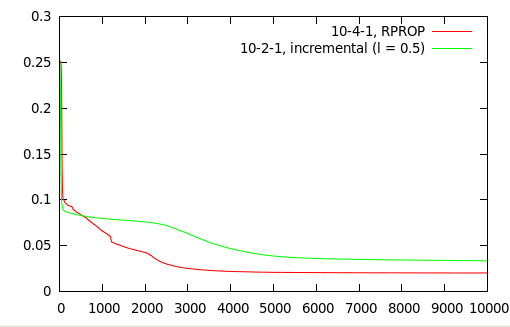
\includegraphics[width=0.85\textwidth]{images/shape-train01-mse}
\label{fig:shape-train-01-mse}
\end{figure}

\begin{figure}[htb]
\caption{Bit fail count through epochs of incremental and RPROP training
for shape matching}
\centering
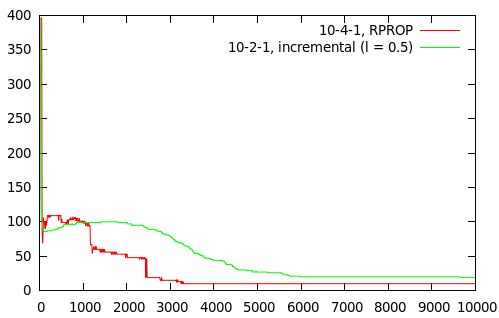
\includegraphics[width=0.85\textwidth]{images/shape-train01-bf}
\label{fig:shape-train-01-bf}
\end{figure}


\begin{figure}[htb]
\caption{Mean square error through epochs of RPROP training for shape matching}
\centering
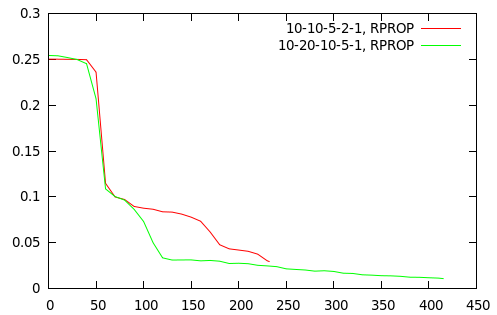
\includegraphics[width=0.85\textwidth]{images/shape-train02-mse}
\label{fig:shape-train-02-mse}
\end{figure}

\begin{figure}[htb]
\caption{Bit fail count through epochs of RPROP training for shape matching}
\centering
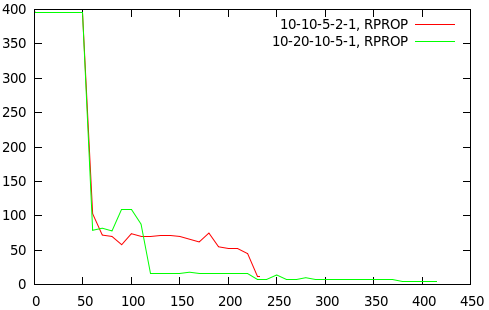
\includegraphics[width=0.85\textwidth]{images/shape-train02-bf}
\label{fig:shape-train-02-bf}
\end{figure}

\subsection{Color matching probability computation}

In order to train and test the artificial neural network for computing color
matching probabilities, the training and test data with the properties shown
in table \ref{table:color-data-properties} were used.

%TODO Pozicioniranje

\begin{table}[h] \begin{center} {\footnotesize
\begin{tabular}{c|c|c|c|c|c}
Data set & groups & different images & positive & negative & positive (\%) \\
\hline
Train & 8 & 43 & 272 & 272 & 0.5 \\
Test & 8 & 36 & 182 & 182 & 0.5 \\
\end{tabular} }
\end{center}
\caption{\footnotesize Properties of training and test data set for color
discrimination}
\label{table:color-data-properties}
\end{table}

Unlike the case with shape discrimination, where the network has been
successfully trained to compute the matching probabilities correctly for the
data in training set, this was not the case with color. Training the network for
color discrimination was unsuccessful; the reliability for training data set
is around $0.7$, while for test data set it is around $0.35$, a seen from table
As seen in table \ref{table:color-training-results}. The training performance is shown in
figures \ref{fig:color-train-01-mse}, \ref{fig:color-train-01-bf}, 
\ref{fig:color-train-02-mse}, \ref{fig:color-train-02-bf}.

\begin{table}[h]
\begin{center} {\footnotesize
\begin{tabular}{|c|c|c||c|c|c||c|c|c|}
\hline
\multicolumn{3}{|c||}{network description} & 
\multicolumn{3}{c||}{training data set} & 
\multicolumn{3}{c|}{testing data set} \\
\hline
neurons & training & learning & MSE & $b$ & $\rho$ & MSE & $b$ & $\rho$ \\ 
by layer & algorithm & rate    & & & & & & \\
\hline

14-1-1 & incremental & 0.9 & 
0.158978 & 122 & 0.776 & 
0.312611 & 201 & 0.448 \\

14-2-1 & incremental & 0.4 & 
0.139997 & 177 & 0.675 & 
0.17183 & 246 & 0.324 \\

14-10-10-1 & RPROP & - & 
0.14981 & 193 & 0.645 & 
0.165843 & 256 & 0.297 \\

14-15-10-2-1 & RPROP & - & 
0.184827 & 89 & 0.836 & 
0.260222 & 222 & 0.390 \\

\hline
\end{tabular} }
\end{center}
\caption{\footnotesize Properties of training and test data set for color
discrimination}
\label{table:color-training-results}
\end{table}

\begin{figure}[htb]
\caption{Mean square error through epochs of incremental training
for color matching, with different training data}
\centering
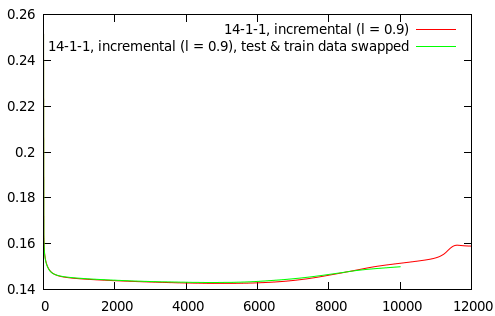
\includegraphics[width=0.85\textwidth]{images/color-train01-mse}
\label{fig:color-train-01-mse}
\end{figure}

\begin{figure}[htb]
\caption{Bit fail count through epochs of incremental training
for color matching, with different training data}
\centering
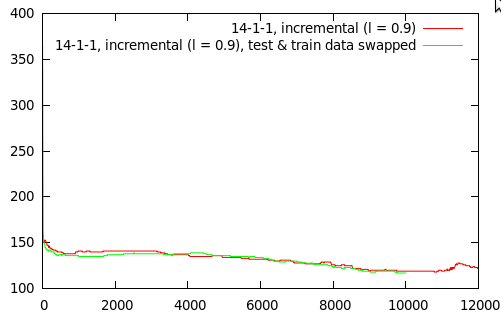
\includegraphics[width=0.85\textwidth]{images/color-train01-bf}
\label{fig:color-train-01-bf}
\end{figure}


\begin{figure}[htb]
\caption{Mean square error through epochs of RPROP training for color matching}
\centering
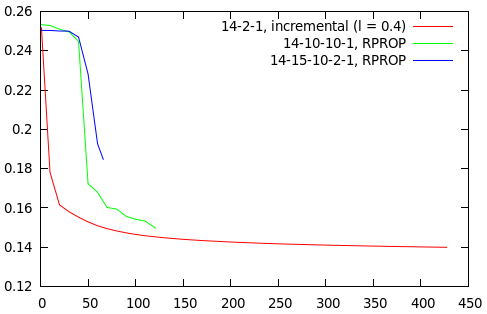
\includegraphics[width=0.85\textwidth]{images/color-train02-mse}
\label{fig:color-train-02-mse}
\end{figure}

\begin{figure}[htb]
\caption{Bit fail count through epochs of RPROP training for color matching}
\centering
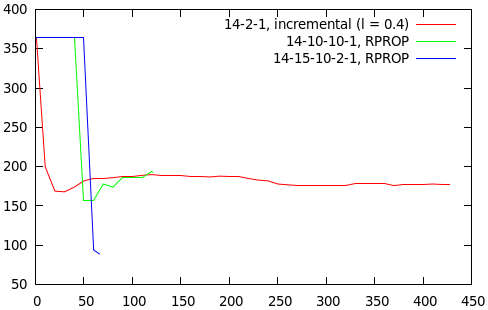
\includegraphics[width=0.85\textwidth]{images/color-train02-bf}
\label{fig:color-train-02-bf}
\end{figure}

\subsection{Plate matching probability computation}

To train and test the artificial neural network for computing the match
probability of the licence plate images, the training and test data with the
properties shown in table \ref{table:plate-data-properties} were used.

\begin{table}[h]
\begin{center} {\footnotesize
\begin{tabular}{c|c|c|c|c|c}
Data set & groups & different images & positive & negative & positive (\%) \\
\hline
Train & 16 & 51 & 144 & 144 & 0.5 \\
Test & 15 & 43 & 102 & 102 & 0.5 \\
\end{tabular} }
\end{center}
\caption{\footnotesize Properties of training and test data set for plate
discrimination}
\label{table:plate-data-properties}
\end{table}

The training performance of the network is shown in figures
\ref{fig:plate-train-mse} and \ref{fig:plate-train-bf}. It can be seen
that, regardless of the training algorithm used, the network is easily trained.

The precise results are shown in table \ref{table:plate-training-results}.
As it can be seen from the table, the network is able
to achieve a reliability of around $0.98$ for training data set and a
reliability of around $0.4$ for test data set.

\begin{table}[h]
\begin{center} {\footnotesize
\begin{tabular}{|c|c|c||c|c|c||c|c|c|}
\hline
\multicolumn{3}{|c||}{network description} & 
\multicolumn{3}{c||}{training data set} & 
\multicolumn{3}{c|}{testing data set} \\
\hline
neurons & training & learning & MSE & $b$ & $\rho$ & MSE & $b$ & $\rho$ \\ 
by layer & algorithm & rate    & & & & & & \\
\hline

32-1-1 & RPROP & - & 
0.0204451 & 6 & 0.979 & 
0.552851 & 114 & 0.441 \\

32-20-1 & Quickprop & 0.4 & 
0.0211049 & 6 & 0.979 & 
0.545 & 123 & 0.397 \\

32-1-1 & incremental & 0.3 & 
0.0207712 & 6 & 0.979 & 
0.581113 & 142 & 0.304 \\

32-20-15-1 & RPROP & - & 
0.0204469 & 6 & 0.979 & 
0.495208 & 104 & 0.490 \\

\hline
\end{tabular} }
\end{center}
\caption{\footnotesize Properties of training and test data set for plate
discrimination}
\label{table:plate-training-results}
\end{table}

\begin{figure}[htb]
\caption{Mean square error through epochs of training for plate matching}
\centering
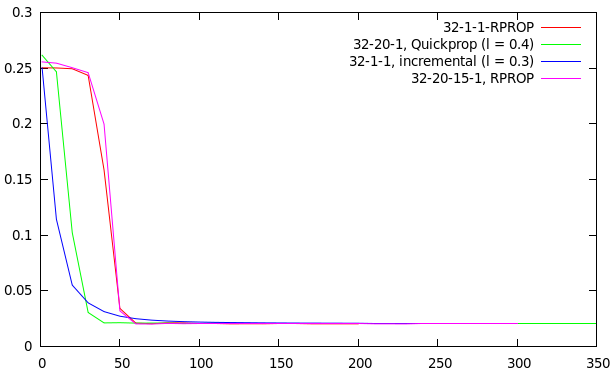
\includegraphics[width=0.85\textwidth]{images/plate-train-mse}
\label{fig:plate-train-mse}
\end{figure}

\begin{figure}[htb]
\caption{Bit fail count through epochs of training for plate matching}
\centering
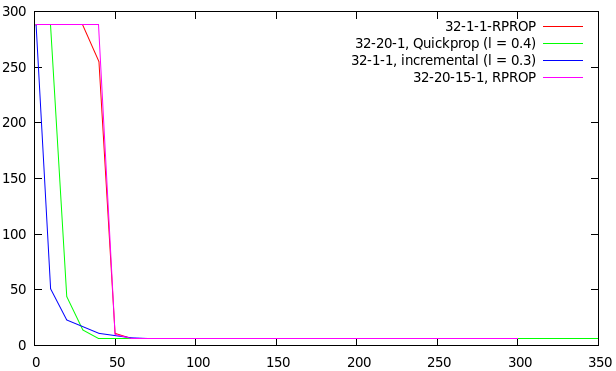
\includegraphics[width=0.85\textwidth]{images/plate-train-bf}
\label{fig:plate-train-bf}
\end{figure}



\chapter{Conclusion}
Based on the experimental results presented in the previous section, a number of
inferences can be made. First, statistical analyses of the matching
discriminators show that some of them look promising for use in image matching. These primarily
include perimeter quotient, portion of hue-dominant pixels, average saturation,
and discriminators derived from observing properties of black components, i.e.
characters, in the licence plate region of the image. Second, when matching
discriminator values are used as inputs in artificial neural networks,
especially in the case of plate discriminators, it is clearly visible that the
artificial neural network can be trained to work well with the training set,
even if only one or two hidden neurons are used. 

Because of the fact that good training performance is achieved even if a small
number of hidden neurons are used, the possibility that the network is overfit
and thus unable to work well with a previously unseen data set is reduced to
minimum. This leads to a conclusion that the size of the training data set was
too small to ensure that an artificial neural network is able to extract the
information necessary to do the matching discrimination.

Finally, in section \ref{section:matching-algorithm} the matching
has been successfully reduced to an assignment problem which is then
solved by the Hungarian algorithm. Because of its polynomial time, its
application is possible in speed limit detection systems.

\bibliographystyle{plainnat}
\bibliography{biblio}
\graphicspath{images//}

\end{document}
